\section{Ablation Studies}
\label{sec:ablation}

%In our main ablation studies, we systematically evaluate how model size, training temperature, and backbone architecture affect AutoBool's query generation effectiveness. Unless otherwise specified, all models are trained on the same data using our reward function with \(\alpha = 1\). Appendix~\ref{appendix:retrieval_reward} provides comprehensive ablations on reward function design, including the necessity of logarithmic scaling, recall dependency, and precision weighting, as well as sensitivity analyses for the scaling factor M, smoothing constant s, and penalty values. The key finding was that the reasoning based prompt benefit from all of the different reward function component and was robust to different parameter settings. In contrast, the non-reasoning based prompt can be sensitive and therefore does necessitate careful consideration of parameter settings. 

In our main ablation studies, we systematically evaluate how model size, training temperature, and backbone architecture affect AutoBool's query generation effectiveness~\footnote{Unless otherwise specified, all models are trained on the same data using our reward function with \(\alpha = 1\).}.  Appendix~\ref{appendix:retrieval_reward} provides comprehensive ablations on reward function design, including logarithmic scaling, recall dependency, precision weighting, and sensitivity analyses for scaling factor M, smoothing constant s, and penalty values. The key finding is that 
while every component in the retrieval reward is important, reasoning-based prompts are more robust when hyperparameters vary, whereas no-reasoning prompts are more sensitive and require careful selection of hyperparameter values.


\subsection{Effect of Backbone Size}

To understand the impact of backbone model size on retrieval performance, we evaluate Qwen3 models at four parameter sizes (1.7B, 4B, 8B, and 14B), each trained with the same reinforcement learning setup. Figure~\ref{fig:model-size-comparison} shows that increasing model size leads to a consistent improvement in F\textsubscript{3}, reflecting better overall balance between recall and precision. However, this comes with a trade-off: recall and recall-threshold metrics (recall > 80\%, recall > 90\%) tend to decrease slightly as model size increases. This suggests that larger models may learn to generate more screening-efficient queries, retrieving fewer documents with higher precision, at the cost of missing some relevant studies.

These findings highlight the importance of aligning model scale with task priorities. For high-recall applications like systematic reviews, smaller models (e.g., 4B) may be preferable due to their stronger recall performance. In contrast, larger models (e.g., 8B or 14B) may be more appropriate when minimizing screening effort is critical and slight recall reductions are acceptable.

\subsection{Impact of Temperature}

\begin{figure*}[htbp]
	\centering
	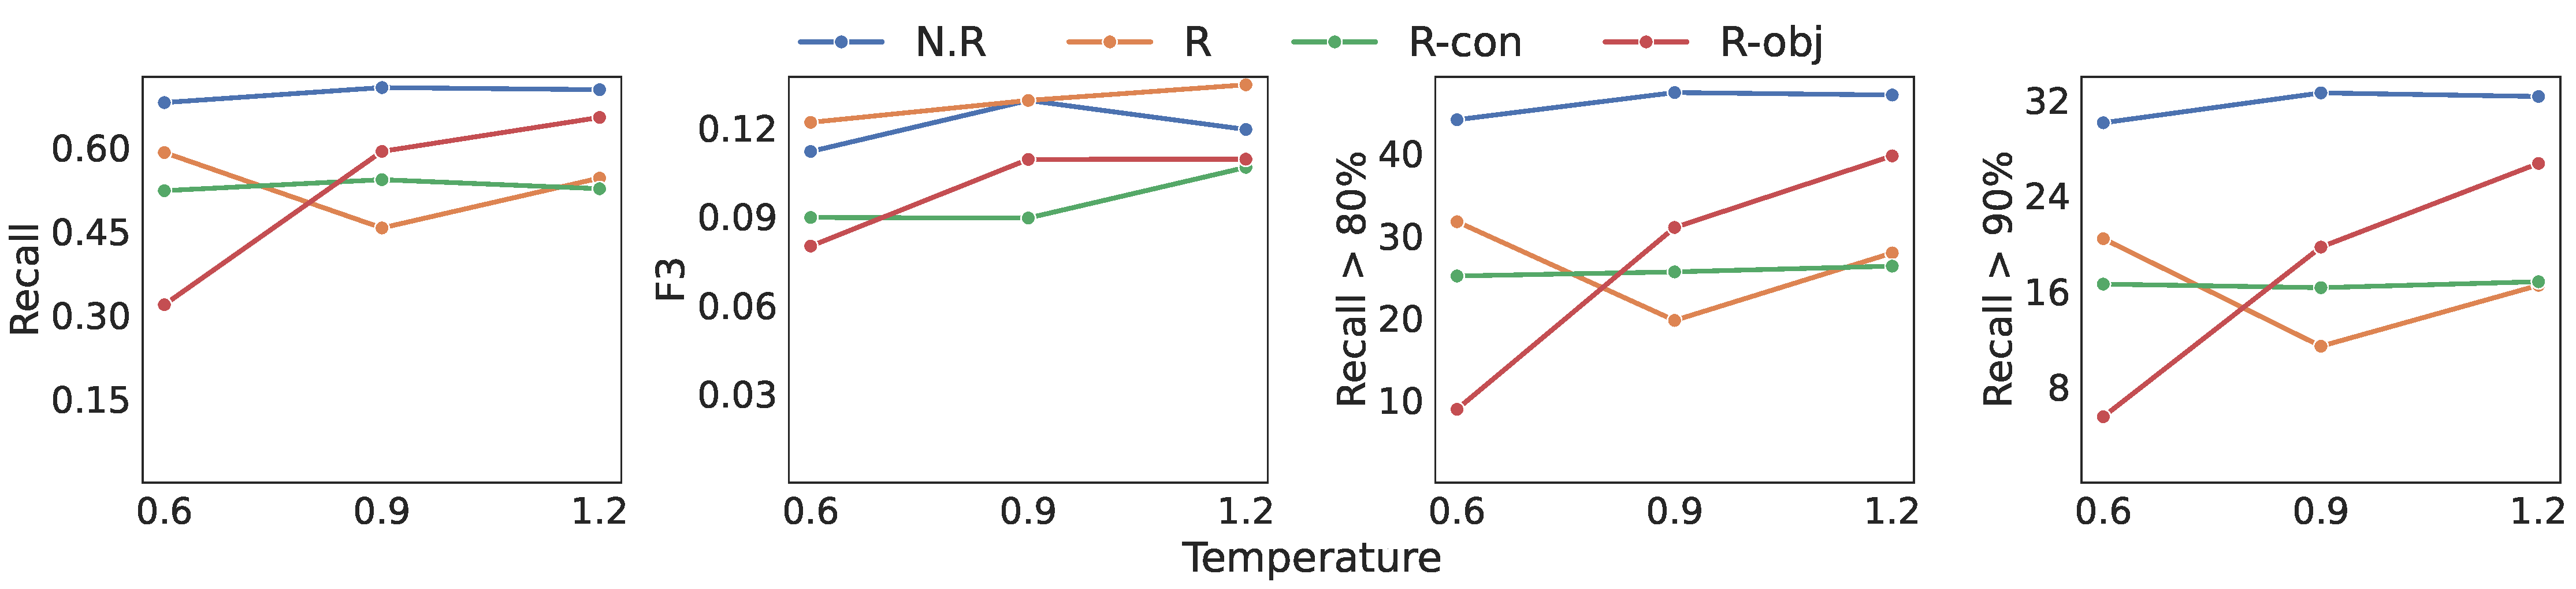
\includegraphics[width=\textwidth]{figures/temperature_performance_plot_final.pdf}
	\caption{Effect of reinforcement learning training temperature value on the effectiveness of Boolean query generation across prompt types on the PubMed Temporal-Cutoff set,  all result based on Qwen3-4B Model.}
	\label{fig:temperature-comparison}
\end{figure*}

At training time, the generation temperature controls sampling diversity: higher values promote more varied outputs, while lower values encourage more deterministic decoding during training for the same topic. To assess its effect on retrieval effectiveness, we evaluate AutoBool models at three generation temperatures: 0.6, 0.9, and 1.2.
As shown in Figure~\ref{fig:temperature-comparison}, increasing temperature consistently improves all primary metrics. This indicates that more diverse generations help the model explore effective query formulations, resulting in broader coverage and higher-quality retrieval.


\subsection{Effect of Backbone Model }

\begin{table}[t]
	\centering
	\footnotesize
	\caption{Impact of Backbone model on the effectiveness of Boolean query generation across prompt types on the PubMed Temporal-Cutoff set.}
	\renewcommand{\arraystretch}{1.25}
	\label{tab:model_comparison}
		\begin{tabular*}{\columnwidth}{@{\extracolsep{\fill}}llcccc@{}}
			\toprule
			Model & Prompt & Recall & F3 & \parbox{2.5em}{Recall\\>80\%} & \parbox{2.5em}{Recall\\>90\%} \\
			\midrule
			\multirow{4}{*}{\rotatebox{90}{Qwen3-8B}} & N.R & 0.7116 & 0.1304 & 47.90 & 32.80 \\
			& R & 0.4716 & 0.1360 & 20.80 & 13.20 \\
			& R-con & 0.4928 & 0.1167 & 22.50 & 14.40 \\
			& R-obj & 0.5097 & \textbf{0.1376} & 19.50 & 12.30 \\
			\midrule
			\multirow{4}{*}{\rotatebox{90}{Llama3.1-8B}} & N.R & \textbf{0.7380} & 0.1035 & 53.00 & 38.00 \\
			& R & 0.7375 & 0.0999 & \textbf{54.20} & \textbf{39.70} \\
			& R-con & 0.7165 & 0.1006 & 48.60 & 34.00 \\
			& R-obj & 0.7291 & 0.1075 & 51.40 & 36.60 \\
			\bottomrule
		\end{tabular*}%

\end{table}


To examine how the backbone model impacts effectiveness, we compare two similarly sized models—Qwen3-8B and LLaMA3.1-8B—trained with identical reinforcement learning procedures. Table~\ref{tab:model_comparison} shows that LLaMA3.1-8B consistently outperforms Qwen3-8B across all primary recall metrics.
LLaMA3.1-8B obtains the highest recall across all prompt types, with strong results under \texttt{N.R} (0.7380 recall, 53.00\% recall > 80\%) and \texttt{R} (0.7375 recall, 54.20\% recall > 80\%). In contrast, Qwen3-8B yields higher F\textsubscript{3}, suggesting greater efficiency in reducing screening effort.

Consistent with findings on Qwen models, LLaMA3.1 is also more effective under the \texttt{No Reasoning} prompt, indicating that post-training, simpler prompting leads to more effective generation. Reasoning-based prompts tend to degrade recall performance, though they may still offer benefits in terms of robustness or interpretability.

Overall, these results highlight that backbone differences among decoder-only LLMs can significantly influence learning dynamics under reinforcement optimization, particularly in how recall and efficiency are balanced during query generation.